\documentclass[main.tex]{subfiles}

\begin{document}
\sloppy


\vspace{1.0cm}

\chapter{Primi Task}\label{sec:Primi Task}
Come accennato nel capitolo \ref{Tirocinio}, durante il tirocinio mi sono stati assegnati diversi task, sempre più importanti. Tra questi task possiamo individuare i seguenti:
\begin{itemize}
    \item Risolvere problemi riguardanti API precedentemente sviluppate;
    \item Abilitare i linters disattivati;
    \item Design e sviluppo di nuove funzionalità riguardante il salvataggio dei file ottenuti tramite bluetooth;
    \item Progettazione di una simulazione tra bot per verificare il corretto funzionamento dell'applicazione.
\end{itemize}
In questo capitolo verranno analizzati i primi tre tipi di task.

\section{Minor Bug}
La prima tipologia corrisponde ad una serie di piccoli task svolti nel primo mese di tirocinio per prendere dimestichezza con il progetto e gli strumenti usati.\newline
Durante questo primo periodo ho apportato piccole modifiche al progetto per risolvere alcuni task segnalati da altri tirocinanti come \say{minor bug}. 

\subsection{ReadAll in updateMeNickname is deprecated}
Questo primo task richiedeva la rimozione dell'ormai deprecato pacchetto \say{io/ioutil}. \newline
La deprecazione di questo pacchetto è avvenuta con l'aggiornamento 1.16 \cite{Go116} di Go poiché reputato come una \say{raccolta di cose mal definita e difficile da capire}. Per questo motivo ho sostituito tutti gli utilizzi di \textbf{ioutil.ReadAll(r.Body)} con la funzione \textbf{io.ReadAll(r.Body)} del pacchetto \say{io}. \newline

\subsection{Remove github.com/pkg/errors dependency}
Similmente al task precedente, anche il pacchetto \say{github.com/pkg/errors} è risultato obsoleto dopo l'aggiornamento 1.13 \cite{Go113} di Go il quale ha introdotto una nuova gestione degli errori direttamente nella libreria standard di Go. A causa di ciò è risultato necessario rimpiazzare tutti i suoi utilizzi con le funzioni della libreria standard. \newline
Nel dettaglio ho rimpiazzato tutti gli \textbf{errors.New()} ed i \textbf{errors.Wrap()} con \textbf{fmt.Errorf}, rimuovendo così \say{github.com/pkg/errors} completamente.

\section{Enable all linters in `.golang-ci.yml` and fix all issues}
Il progetto di Generocity utilizza diversi linters 
\cite{Linters} per analizzare il codice e segnalare errori, bug, errori stilistici e costrutti sospetti ma al mio arrivo alcuni di questi linters erano disattivati perché aggiunti dopo l'avvio del progetto. Il mio compito è stato quindi di attivare tutti i linters in quel momento disattivati e risolvere tutti i problemi che avrebbero inevitabilmente segnalato nel codice. \newline
Ecco una lista di tutti i linters attivati e di cosa si occupano: 
\begin{itemize}
    \item \textbf{errorlint}: questo linter trova codice che causerà problemi con il wrapping degli errori. Ad esempio l'operazione \say{err == ErrFoo} segnalerà un errore perché comparare wrapped errors con il \say{==} potrebbe non funzionare. Bisogna quindi sostituire tutte queste comparazioni presenti nel codice con la funzione \textbf{errors.Is(err, ErrFoo)};
    \item \textbf{forcetypeassert}: questo linter trova asserzioni di tipo di cui non vengono gestiti gli errori;
    \item \textbf{goconst}: questo linter trova tutte le stringhe che vengono utilizzate molteplici volte, le quali potrebbero quindi essere rese delle costanti;
    \item \textbf{gocritic}: questo linter verifica la presenza di bug, prestazioni e problemi di stile;
    \item \textbf{nestif}: questo linter trova le istruzioni if annidate che rendono il codice difficile da leggere calcolandone la complessità e segnalando quelle che ne hanno una troppo elevata;
    \item \textbf{prealloc}: questo linter trova le dichiarazioni di slice che potrebbero essere potenzialmente preallocate per evitare una riallocazione successiva alla loro creazione;
    \item \textbf{revive}: questo linter fornisce un framework per lo sviluppo di regole personalizzate da applicare al codice. Nel nostro caso revive ha segnalato una grande varietà di errori come il mancato utilizzo del CamelCase nei nomi delle variabili oppure un utilizzo non necessario delle else;
    \item \textbf{unconvert}: questo linter trova conversioni di tipo non necessarie;
    \item \textbf{wastedassign}: questo linter trova istruzioni di assegnazione sprecate.
\end{itemize}


\section{Allow to modify "modes" field in bluetooth file}
L'applicazione, durante un viaggio, raccoglie alcuni dati tramite bluetooth per capire che mezzo di trasporto l'utente stia utilizzando e li immagazzina in un object storage chiamato MinIO. \newline
Col tempo però è risultato necessario un modo per poter modificare i dati immagazzinati nel caso in cui l'applicazione abbia sbagliato nel riconoscere il mezzo utilizzato. \newline

\subsection{Strutture Dati}
Le scansioni effettuate durante un viaggio vengono rappresentate in questa struttura dove:
\begin{itemize}
    \item \textbf{Trip}: l'id del trip da cui sono stati raccolti i dati;
    \item \textbf{Mode}: il mezzo di trasporto su cui si è svolto il viaggio;
    \item \textbf{Scans}: le scansioni effettuate.
\end{itemize}

\lstinputlisting[language=go]{Code/PrimiTask/bluetooth-struct.go}

\subsection{Modifiche al salvataggio dei file}

I dati relativi ad un singolo viaggio venivano salvati in un file JSON dal nome \emph{bluetoothconnections/\textbf{userID}\_\textbf{time}.json} dove \textbf{userID} era l'id dell'utente che ha effettuato il viaggio e \textbf{time} era il timestamp di ricezione dei dati da parte del server.
Salvare i file con questo nome rendeva però impossibile ricercare il file corretto che l'utente ha intenzione di modificare dato che l'applicazione non conosce il tempo preciso in cui il file è stato memorizzato. Ho quindi modificato il nome con cui i file venivano salvati, passando dal vecchio \textbf{userID\_time.json} a \textbf{tripID.json}. In questo modo l'applicazione, per richiedere la modifica di un file, dovrà specificare solo l'id del trip dov'è stato rilevato l'errore. \newline
Oltre ai nomi è risultato anche che al momento del salvataggio dei file non venivano effettuati controlli se il file inserito fosse effettivamente valido. Per effettuare questi controlli ho quindi aggiunto due piccole funzioni a quella di salvataggio dei file.\newline
La funzione \textbf{CheckTripID} controlla che nel database esista realmente un trip con id uguale a quello del trip di cui si stanno salvando le connessioni bluetooth.
\lstinputlisting[language=go]{Code/PrimiTask/check-trip-id.go}

La funzione \textbf{CheckTripUser} controlla che l'utente che sta salvando il file è lo stesso che ha effettuato il trip. \label{CheckTripUser}
\lstinputlisting[language=go]{Code/PrimiTask/check-trip-user.go}


\subsection{Bluetooth-mode-update API}
Ora che esiste un modo per riconoscere i file memorizzati ho potuto realizzare un nuovo endpoint API  \emph{/bluetooth/\{tripid\}/} dove \textbf{tripid} indica l'identificatore del trip da modificare.\newline
L'API usa i seguenti parametri:
\begin{itemize}
    \item \textbf{tripid}: identificativo unico del trip da modificare;
    \item \textbf{mode}: stringa enum che corrisponde al corretto mezzo di trasporto con il quale si è svolto il trip (\say{walk}, \say{metro}, \say{car},\say{tram}, \say{bus} ).
\end{itemize}

\begin{figure}[H]
    \centering
    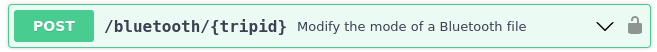
\includegraphics[width=1\linewidth]{img/primi task/update_bluetooth swagger.png}
    \caption{Path bluetooth update API}
    \label{fig:bluetooth update-path}
\end{figure}

\begin{figure}[H]
    \centering
    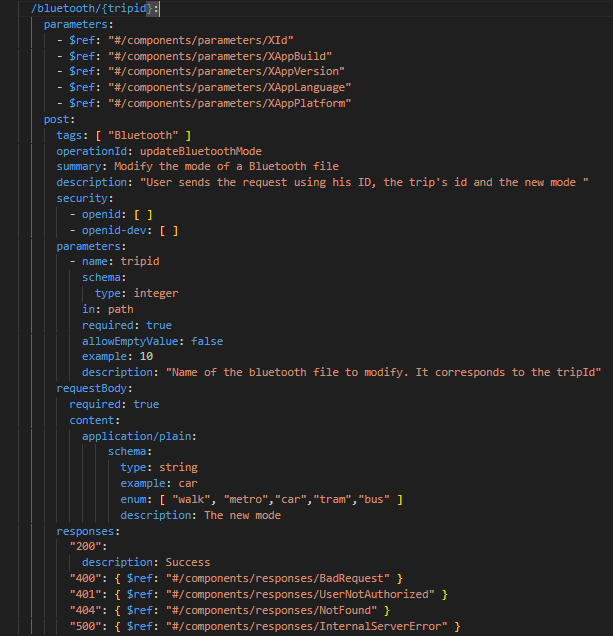
\includegraphics[width=1\linewidth]{img/primi task/api-doc.png}
    \caption{Bluetooth update API documentazione}
    \label{fig:bluetooth update-doc}
\end{figure}


\subsection{Implementazione API}
Ho implementato l'API nella funzione \textbf{updateBluetoothMode}, la quale, dopo aver raccolto i dati, effettua alcuni controlli per verificare la validità della richiesta.\newline

\lstinputlisting[language=go]{Code/PrimiTask/bluetooth-mode-update.go}

Con la funzione \textbf{CheckTripUser} \ref{CheckTripUser}, viene controllato se l'utente che sta facendo la richiesta di modificare il file \emph{filename} è lo stesso utente che ha effettuato quel viaggio ed ha quindi il permesso di modificarlo.\newline
Una volta verificato che il viaggio esiste e che l'utente ha il permesso di effettuare la modifica, viene usata la funzione \textbf{fs.UpdateBluetoothMode}, la quale verifica che il file esista, legge il file, modifica la \emph{Mode} salvata con quella indicata dall'utente e salva la modifica.

\lstinputlisting[language=go]{Code/PrimiTask/fs-bluetooth-update.go}





\end{document}